\documentclass[../../document.tex]{subfiles}

\begin{document}
    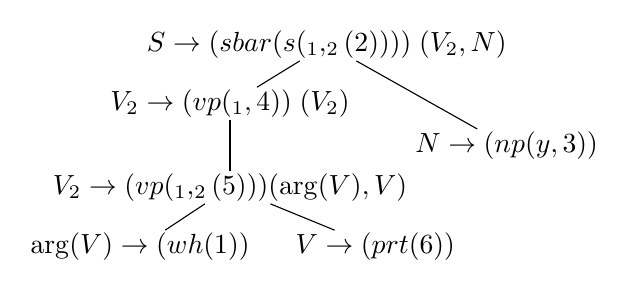
\begin{tikzpicture}[anchor=center, outer sep=0px, inner sep=1pt]
        \node (root) {\(\nt{S} \to (\cn{sbar}(\cn{s} (\x_1, \x_2(\tn{2}))))\;(\nt{V}_2, \nt{N})\)}
        [sibling distance=7em,level distance=5ex]
        child { node (vp1) {\(\nt{V}_2 \to (\cn{vp}(\x_1, \tn{4}))\;(\nt{V}_2)\)}
            [sibling distance=6.5em]
            child{ node[yshift=-2ex] (vp2) {\(\nt{V}_2 \to (\cn{vp}(\x_1, \x_2(\tn{5}))) (\mathrm{arg}(\nt{V}), \nt{V\binsym{}})\)}
                child { node (term0) {\(\mathrm{arg}(\nt{V}) \to (\cn{wh}(\tn{1}))\)}}
                child { node[xshift=2em] (term5) {\(\nt{V\binsym{}} \to (\cn{prt}(\tn{6}))\)}}}}
        child { node[yshift=-3.5ex, xshift=3em] (np) {\(\nt{N} \to (\cn{np}(y, \tn{3}))\)}};
    \end{tikzpicture}
\end{document}